\chapter{总体方案与系统架构}

\section{云—边—端分层设计思想}

CoTriage 面向的不是单机日志分析，而是一个跨越数据产生现场、边缘计算节点与云端智能服务的协同系统。三层所掌握的信息、可使用的资源和必须承担的时限不同：端侧距离设备与故障最近，能够持续感知但不适合承担复杂推理；边缘侧具备稳定的现场算力和局部知识，必须在低时延与弱网条件下维持基本判断；云端拥有更强模型和跨节点上下文，适合处理少量复杂、高风险或认知不确定的事件。因此，系统没有把日志无差别汇聚到一个中心，而是按照“端侧形成可信事件、边缘完成实时分诊、云端提供按需认知增益”的原则分配能力。

这一分层不是静态的数据转发链。边缘侧 RAISE 会同时观察事件价值与系统状态，动态决定事件在本地结束、立即上云或延期发送；云端诊断完成后再将结构化结论与反馈写回。系统由此形成两个相互嵌套的闭环：实时闭环在端—边之间完成持续采集与现场初判，增益闭环在边—云之间完成价值路由、深度诊断和反馈演进。即使增益闭环暂时中断，实时闭环仍应继续运行。

\begin{table}[htbp]
  \centering
  \small
  \caption{云、边、端三层的职责边界与设计目标}
  \label{tab:cloud-edge-end-responsibility}
  \begin{tabularx}{\textwidth}{>{\bfseries}p{0.11\textwidth} p{0.22\textwidth} X X}
    \toprule
    层级 & 典型部署位置 & 核心职责 & 设计目标 \\
    \midrule
    端侧 & 设备、工控机、服务器或业务节点 & 产生原始日志，就近采集并补充稳定来源与时间信息 & 感知连续、开销轻量、原始证据不丢失 \\
    边缘侧 & 工厂、园区或站点近端计算节点 & 事件流承载、分层推理、RAISE 决策、Outbox 与本地结果输出 & 低时延自治、资源受控、弱网可用、决策可解释 \\
    云端 & 中心集群、云服务或大模型 Provider & 跨来源上下文聚合、脱敏、深度诊断、反馈写回与统一治理 & 按需调用、全局关联、诊断增益、集中管理 \\
    \bottomrule
  \end{tabularx}
\end{table}

\section{总体架构与协同主链}

\begin{figure}[htbp]
  \centering
  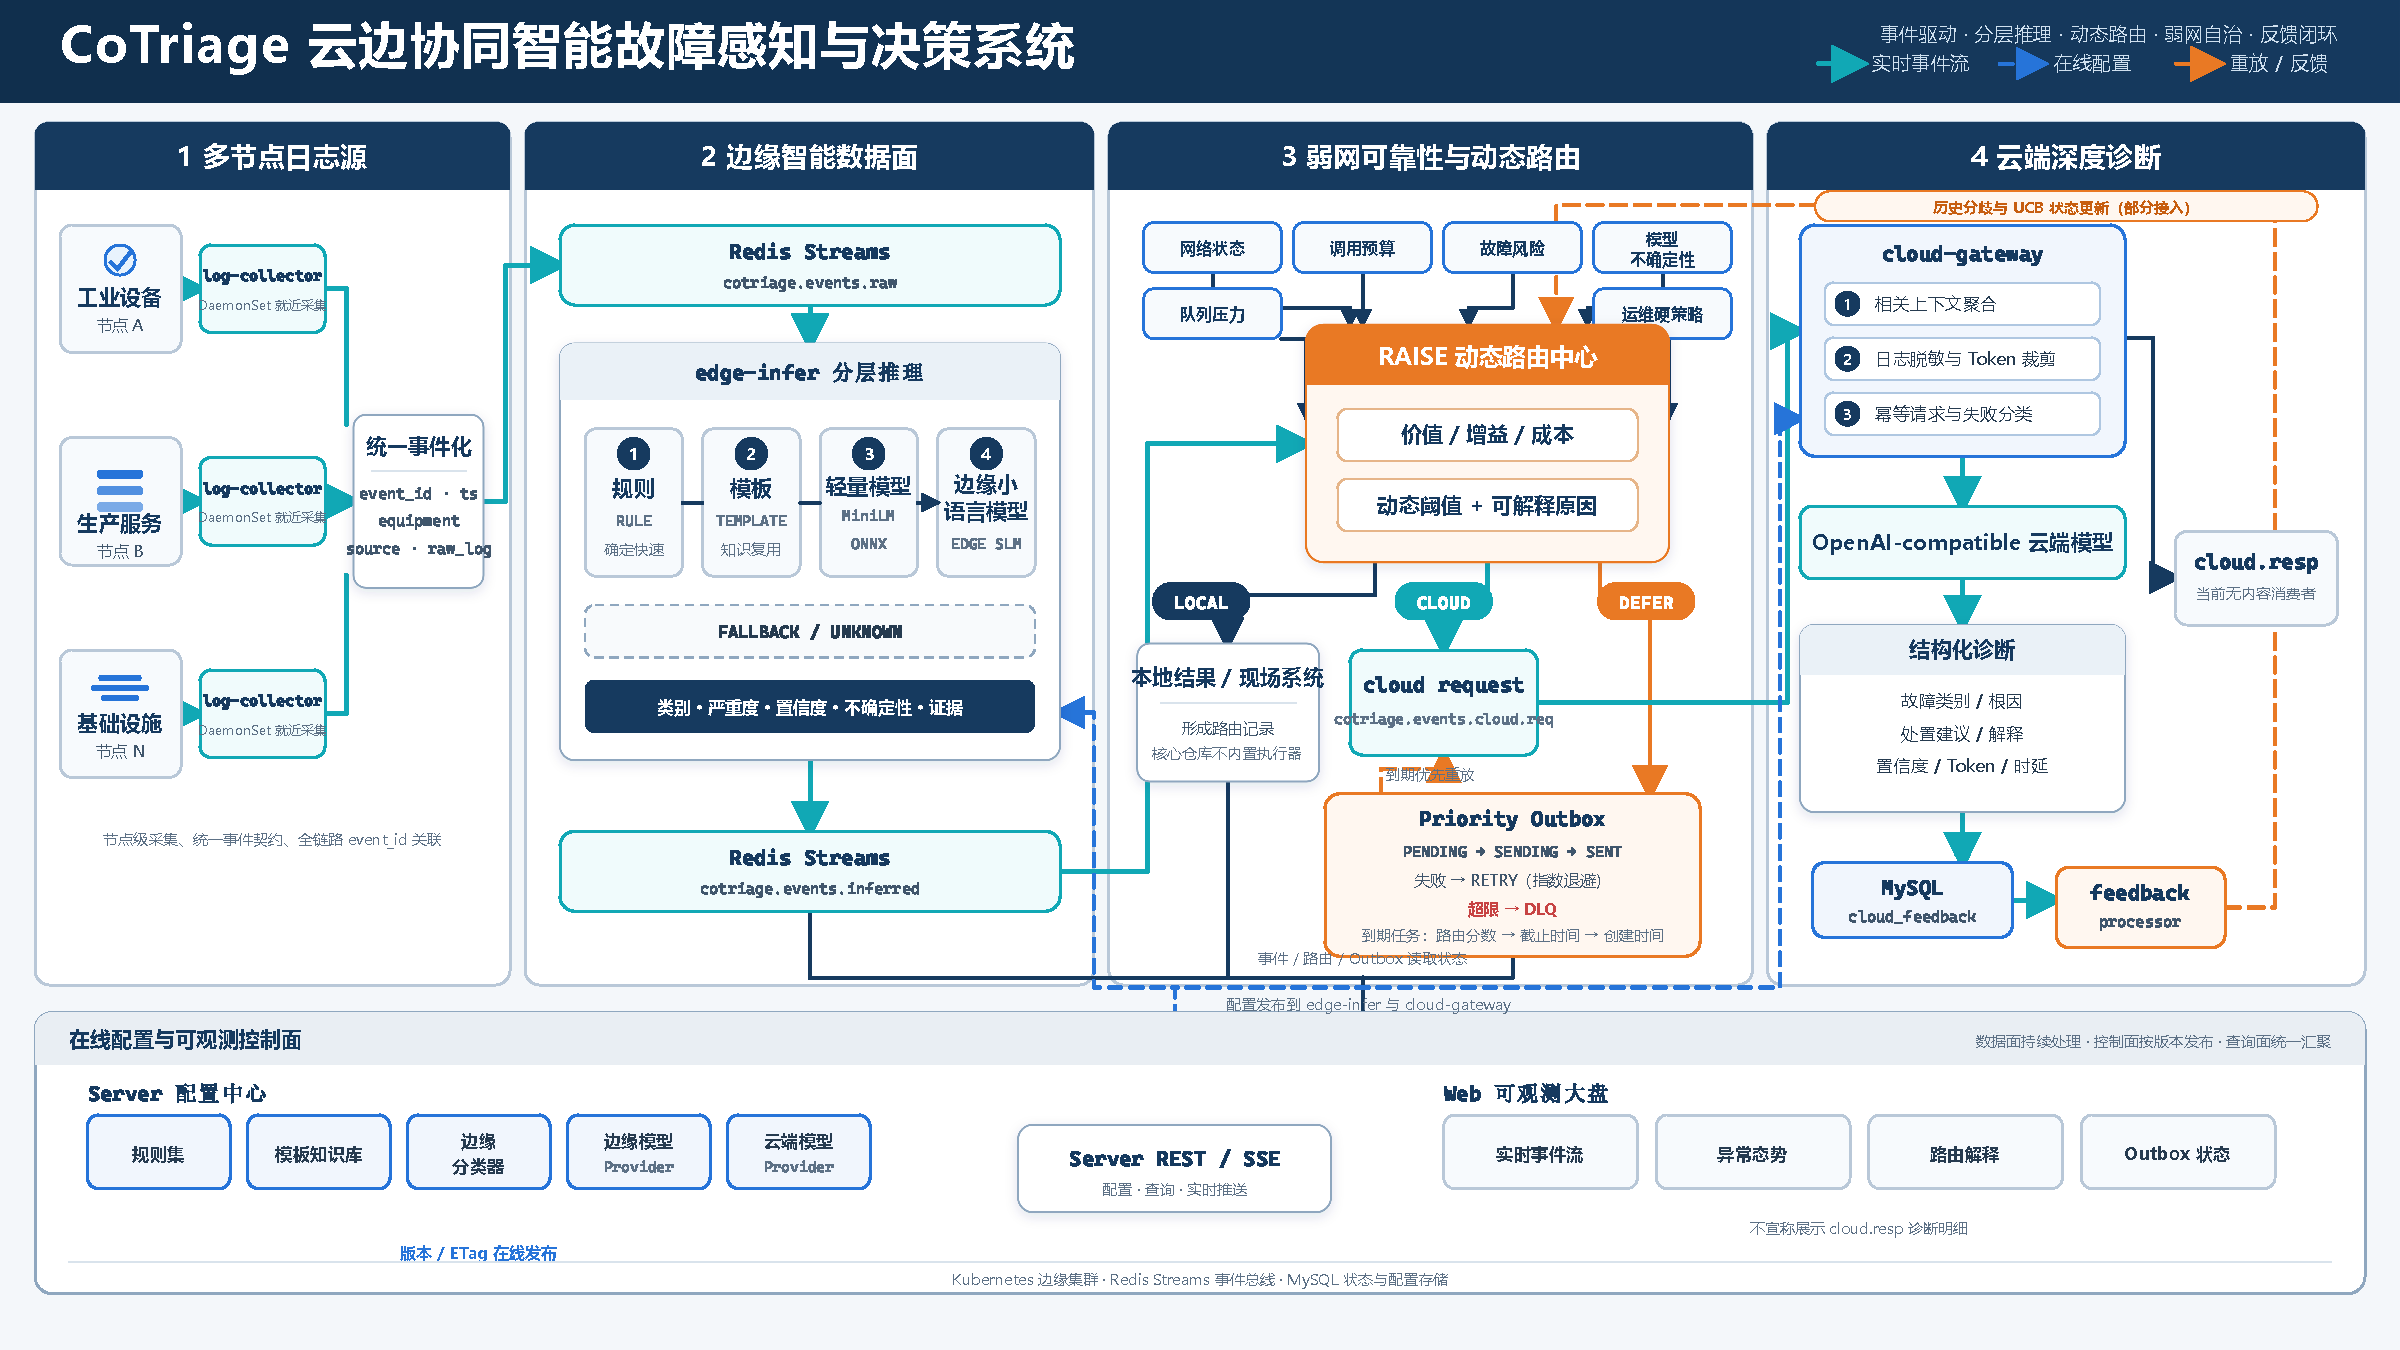
\includegraphics[width=\textwidth]{figures/cotriage-system-architecture.pdf}
  \caption{CoTriage 云—边—端协同总体架构}
  \label{fig:architecture}
\end{figure}

\cref{fig:architecture}从左至右描述了一条事件如何跨层流动。端侧多个日志源由近端采集器转换为统一事件；边缘侧通过 Redis Streams 解耦持续事件流，依次完成异构分层推理和 RAISE 路由，确定性事件在本地闭环，高价值事件进入云端请求流，暂不可发送的事件进入风险优先 Outbox；云端网关裁剪并脱敏上下文，调用兼容 Provider 生成根因、建议和解释，再把结果持久化并形成反馈。Server 与 Web 组成统一控制和观测入口，贯穿三层但不阻塞后台数据面。

架构中的“协同”体现在三个方面。其一是\textbf{能力协同}：规则、模板、轻量模型、边缘小模型与云端大模型按事件难度逐级使用。其二是\textbf{资源协同}：网络、队列、预算和策略直接进入路由判断，避免云端能力被当作无限资源。其三是\textbf{时间协同}：实时结果与深度结果可以异步产生，Outbox 又把“当前不能发送”转换为“条件恢复后继续分析”，使诊断深度不必与现场响应共用同一时限。

\section{端侧：多源日志感知与可信事件生成}

端侧包括工业设备控制程序、工控机操作系统、Linux 主机、Hadoop 或 ZooKeeper 节点以及 Web 服务等日志产生单元。不同来源的文本格式和业务语义可以不同，但进入协同主链前必须获得共同坐标：稳定事件标识、设备标识、来源、采集时间和原始内容。\texttt{log-collector} 以节点近端方式持续读取新增日志，尽快完成事件化并写入原始事件流，不在采集阶段执行高成本语义判断。

将采集能力放在端侧附近具有三项作用。第一，日志在产生后无需等待跨网传输即可进入处理链，降低现场感知对外部网络的依赖；第二，设备身份在源头绑定，后续跨节点关联不必仅靠正文猜测来源；第三，原始日志可以优先留在边缘域，只有被选中的事件及裁剪上下文才需要跨越云边边界。端侧的职责是持续、轻量、忠实地提供证据，而不是独立完成所有诊断。

端侧发生故障时，系统采用“局部影响、恢复续接”的原则：单个采集实例异常不应阻塞其他节点，恢复后继续读取新增内容；日志来源新增时只扩展采集适配与设备登记，不改变上游推理和路由契约。第 4 章将进一步说明多节点登记、统一事件字段、消息确认与幂等追踪。

\section{边缘侧：实时推理、价值路由与弱网自治}

边缘侧是 CoTriage 的实时决策中心，而不是云端模型的简单转发代理。它部署在工厂、园区或站点近端，由事件总线、\texttt{edge-infer}、\texttt{onnx-classifier}、\texttt{router-controller} 和 Outbox 共同组成，承担“先形成可用判断，再决定是否需要更强能力”的职责。

\subsection{由快到慢的现场推理链}

\texttt{edge-infer} 将规则、模板知识库、MiniLM ONNX 轻量分类器和边缘小语言模型组织为可早停的分层路径。明确告警优先由规则或模板低成本收敛，常见但未命中的语义交给轻量模型，开放性更强的内容再调用边缘小模型。各层输出统一的类别、严重度、置信度、不确定性、证据、推理路径和版本，使后续路由不依赖某一种模型的私有格式。某一模型不可用时，系统保留上一层有效判断并显式记录降级，而不是把服务故障误判为日志正常。

\subsection{RAISE 事件级路由}

边缘推理得到的“当前判断”并不直接等同于最终处理位置。\texttt{router-controller} 通过 RAISE 分离两个问题：事件是否值得获得云端增益，以及此刻是否具备发送条件。前者由风险、不确定性、新颖度、历史边云分歧与跨设备影响共同描述，后者由网络健康、队列压力、调用预算、限流、隐私和运维策略约束。控制器据此输出 \texttt{LOCAL}、\texttt{CLOUD} 或 \texttt{DEFER}，并保存分数、动态门槛、原因和系统快照。

\subsection{弱网条件下的连续运行}

\texttt{LOCAL} 事件直接形成可供现场系统消费的结果；\texttt{CLOUD} 事件进入云端请求流；\texttt{DEFER} 事件先写入 MySQL Outbox，按风险优先级和到期时间重试，超过边界后进入死信治理。由此，断网不会阻塞端—边实时闭环，高价值事件也不会因为一次发送失败永久失去深诊机会。Redis Streams 的追加日志和消费组机制用于解耦边缘各阶段\cite{redisstreams}，MySQL 则保存需要跨重启恢复的路由、Outbox 和状态快照。

\section{云端：跨节点上下文与大模型深度诊断}

云端只接收边缘选择出的高价值事件，不承担全量原始日志的同步处理。\texttt{cloud-gateway} 以主事件为中心，从可用事件中筛选时间邻近、同源、同模板和跨设备关联上下文，对主日志与关联原文执行脱敏，并在 Token 预算内构造诊断请求。云端 Provider 通过 OpenAI-compatible 接口按需接入，使模型可以替换而不改变边缘事件与路由契约。

云端目标不是再次输出一个分类标签，而是把全局信息增量转化为结构化结果：根因候选回答最可能的故障起点，处置建议给出优先检查和操作方向，诊断解释说明采用了哪些现象与关联证据。结果以事件标识和幂等键持久化，避免重试产生重复高成本调用；随后形成纠错、信息增量或高风险确认等反馈，写回事件状态与在线统计，为后续策略演进提供依据。

Server 与 Web 主要部署在中心控制域，提供 REST/SSE、设备和模型配置、运行状态查询与可视化。控制面可以改变规则、模板、模型 Provider 和运维策略，观测面可以展示实时事件、异常态势、路由解释、Outbox 和诊断结果，但两者短时不可用不应停止端侧采集与边缘处理。云端因而同时承担“深度智能中心”和“统一治理中心”两种角色，二者通过接口与实时数据面解耦。

\section{跨层协同：数据流、控制流与反馈流}

云—边—端架构要稳定运行，仅有一条向上的日志流并不够。CoTriage 将跨层通信划分为三类方向不同、时限不同的通道，避免管理操作、实时事件与模型反馈相互阻塞。

\begin{table}[htbp]
  \centering
  \small
  \caption{云、边、端之间的三类协同通道}
  \label{tab:cross-layer-flows}
  \begin{tabularx}{\textwidth}{>{\bfseries}p{0.15\textwidth} p{0.19\textwidth} X X}
    \toprule
    通道 & 主要方向 & 承载内容 & 时限与失败处理 \\
    \midrule
    实时数据流 & 端侧 $\rightarrow$ 边缘侧 & 原始事件、推理事件、本地结果和路由记录 & 持续处理；云端故障不得阻塞端—边主链 \\
    按需诊断流 & 边缘侧 $\leftrightarrow$ 云端 & 已选事件、裁剪上下文、结构化诊断与反馈 & 异步完成；发送受限时进入 Outbox，调用幂等 \\
    控制与观测流 & 云端 $\leftrightarrow$ 边缘／端侧 & 设备、规则、模板、模型、策略、健康与运行状态 & 配置原子生效；失败沿用上一有效版本，观测中断不影响数据面 \\
    \bottomrule
  \end{tabularx}
\end{table}

统一事件是三类通道之间的公共语言。事件标识串联原文、推理、路由和诊断，幂等键约束跨层重试的副作用，规则与模型版本说明当时使用了哪一份能力，路由快照则保留当时的网络、队列、预算与门槛。系统由此不仅能回答“结果是什么”，还能还原“哪一层做了什么、为什么跨层、失败后如何继续”。

\section{端到端事件闭环与部署边界}

一条事件在端侧生成后进入 \texttt{CREATED}，完成边缘推理后转为 \texttt{INFERRED}，形成 RAISE 动作后进入 \texttt{ROUTED}。\texttt{LOCAL} 在边缘结束实时链路；\texttt{CLOUD} 进入云端深诊；\texttt{DEFER} 先进入 Outbox，条件满足后再上云。云端响应最终与原事件关联，并写回诊断与反馈状态。这个生命周期允许事件早停、异步补充和失败重试，不要求所有日志经过完全相同的计算路径。

\begin{table}[htbp]
  \centering
  \footnotesize
  \caption{主要组件在云—边—端架构中的部署与扩展方式}
  \label{tab:layered-components}
  \begin{tabularx}{\textwidth}{>{\bfseries}p{0.10\textwidth} >{\ttfamily}p{0.20\textwidth} X X}
    \toprule
    层级 & \normalfont\bfseries 组件 & 典型部署方式 & 独立扩展依据 \\
    \midrule
    端侧 & log-collector & 按节点部署，生产环境可采用 DaemonSet 或独立采集进程 & 日志来源数量与单节点产生速率 \\
    边缘 & edge-infer / onnx-classifier & 站点近端 Deployment 或本地模型服务 & 事件吞吐、模型时延与边缘资源 \\
    边缘 & router-controller & 独立持续处理组件，连接 Redis 与 MySQL & 路由吞吐、Outbox 规模与重试压力 \\
    云端 & cloud-gateway & 独立 Deployment，通过兼容接口访问 Provider & 云端并发、限流、Token 与预算 \\
    云端 & server / web & 控制与查询服务、Web 服务 & API、SSE 连接和管理访问量 \\
    \bottomrule
  \end{tabularx}
\end{table}

各组件通过统一事件、Redis Streams、HTTP 和 MySQL 状态协作，并可由 Kubernetes 执行声明式部署与独立扩缩容\cite{kubernetes}。当前实现边界也保持明确：\texttt{LOCAL} 结果提供给外部现场系统消费，仓库不内置真实生产处置执行器；Outbox 采用到期扫描重放，尚未由网络恢复信号直接触发；云端反馈已进入统计和状态快照，学习增益尚未自动改写在线路由评分。明确这些边界既避免把演示能力夸大为生产闭环，也为后续工程化提供清晰方向。

后续章节将沿云—边—端主链逐层展开：第 4 章说明端侧多节点采集与统一事件化，第 5 至第 6 章说明边缘分层推理、RAISE 与弱网补偿，第 7 章说明云端上下文诊断和反馈闭环，第 8 章说明统一治理与产品化展示。
